本研究では,
二次元画像データ(RGB)のピクセル値を縦方向($y$方向)にすべて足し合わせて一次元画像をつくる.
それらを並べたものを1次元画像ベクトル$\vec{u}$とする(\ref{eq:onedimension}式参照).

具体的に記述する.
カメラで撮影するのは$320 \times 240$のサイズのピクセル値であるが,不要な部分を切り取って,
約130行目から200行目を切り出す.
コースの壁や障害物となる走行ロボット以外が撮影されている上下の部分を不要な部分とみなす.
つまりコース以外とロボット自身が映ってる部分をトリミングする(Fig.\ref{roboteye}参照).


その画像データのRed,Green,Blueそれぞれのピクセル値を要素としてもつ数値行列を
$\boldsymbol R,\boldsymbol G,\boldsymbol B$とする.
下記のように1次元画像$\vec{u}$を作成する.

\vspace{-2mm}
\begin{eqnarray}
\left\{
\begin{aligned}
\vec u_{\rm R}= \sum_{y=1}^N \boldsymbol R_{y}\\
\vec u_{\rm G}= \sum_{y=1}^N \boldsymbol G_{y}\\
\vec u_{\rm B}= \sum_{y=1}^N \boldsymbol B_{y}\\
\vec u = (\vec u_{\rm R}, \vec u_{\rm G}, \vec u_{\rm B}) \\
\end{aligned}
\right.
\label{eq:onedimension}
\end{eqnarray}
ただし,$\boldsymbol R_y, \boldsymbol G_y, \boldsymbol B_y$は
それぞれ$\boldsymbol R, \boldsymbol G, \boldsymbol B$の第$y$行だけを取り出したベクトルである.
$N$は列の数(本研究では$N$=320),$\vec u$は$960$列のベクトルとなる.


\subsubsection{大きいハンドルで教師データ収集}
教師データは,コースに障害物(他のロボット,Fig.\ref{data_colle}の黒い円囲まれてないロボット)をコースの中にランダムに置いて,
データ収集ロボットをラジコンして,障害物と壁を避けながら時計回りと反時計回り両方走行して,教師データ収集する.
障害物の位置もランダムに変更して,合計3000個教師データ収集した.

ラジコンの方法はtable\ref{radio_rule}の大きいハンドルの部分を参照して,
"D"以外のボタンを押す瞬間の画像データを一次元画像データに変更して,
ソケット通信で学習用パソコンに送信して,教師データの収集を行う.
大きいハンドルというのは,ボタン"J"と"L"押すと,
モーターの出力が35単位変えるということである.
\subsubsection{小さいハンドルで教師データ収集}
小さいハンドルで教師データ収集は大きいハンドルで教師データ収集と同じコースで収集する
,障害物については,止まってるロボット約6台,感覚運動写像より走行するロボット1台,
別の人がラジコンするロボット2台の環境で,データ収集ロボットをラジコンして,
障害物と壁を避けながら時計回りと反時計回り両方走行して,教師データ収集する.
合計6000個教師データ収集した.

ラジコンの方法はtable\ref{radio_rule}の小さいハンドルの部分を参照して,
ボタンを押す瞬間の画像データを一次元画像データに変更して,
ソケット通信で学習用パソコンに送信して,教師データの収集を行う.
小さいハンドルというのは,ボタン"J"と"L"押すと,モーターの出力が15単位変えるということである.

\begin{table}[!ht]
\setlength\tabcolsep{1pt}
\begin{center}
\begin{tabular}{|c|c|c|c|c|}
\hline
 & \multicolumn{2}{|c|}{小さいハンドル} & \multicolumn{2}{c|}{大きいハンドル}\\
\hline
 & Left motor & Right motor & Left motor & Right motor \\
\hline
W & +20 & +20 & +35 & +35\\
\hline
S & -15 & -15 & -35 & -35\\
\hline
A & * & * & -56 & -56\\
\hline
D & * & * & =0 & =0 \\
\hline
J & -15 & +15 & -0 & +35 \\
\hline
L & +15 & -15 & +35 & -0 \\
\hline
K & \multicolumn{4}{|c|}{操作JとKで変化した出力が0になる} \\
\hline
\end{tabular}
\end{center}
\caption{
大きいハンドルと小さいハンドルの違い
}
\label{radio_rule}
\end{table}



\vspace{-2mm}
\begin{figure}[h]
        \centering
        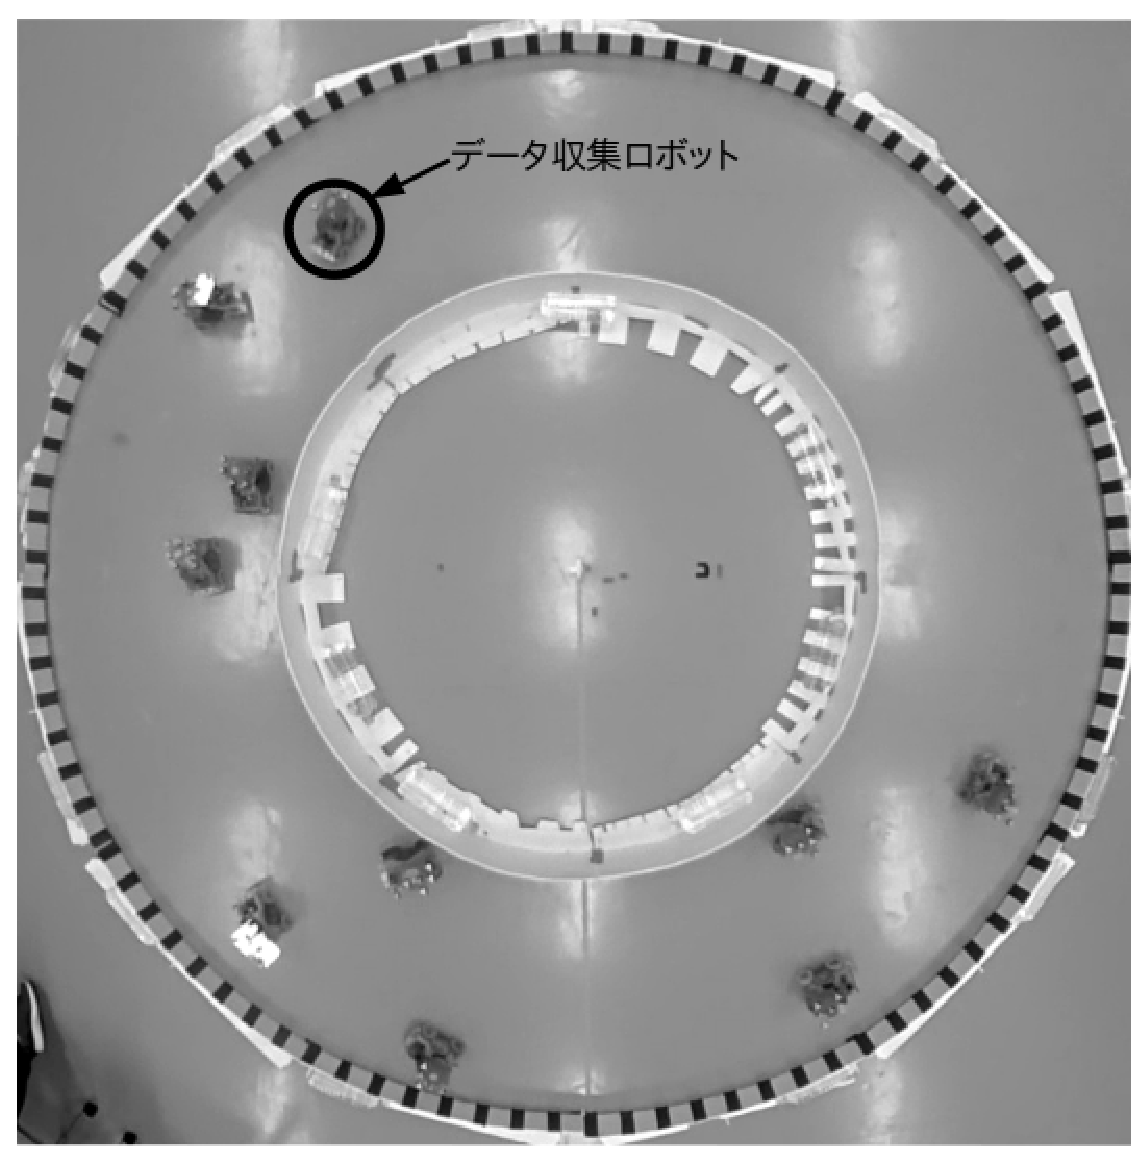
\includegraphics[width=0.8\linewidth]{teacher_collection.eps}
        \caption{データ収集}
        \label{data_colle}
\end{figure}

\vspace{-5mm}
\begin{figure}[h]
\centering
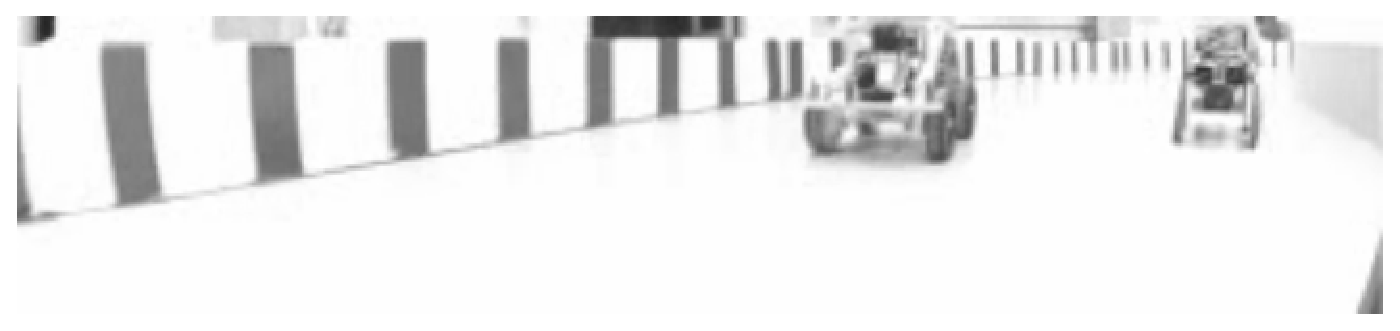
\includegraphics[width=0.7\linewidth]{robot_eye.eps}
\caption{ロボットの視点}
\label{roboteye}
\end{figure}



